\documentclass[11pt,letterpaper]{article}
\usepackage[margin=2.5cm,top=3.5cm,bottom=3cm]{geometry}
\usepackage{booktabs}
\usepackage{graphicx}
\usepackage[hidelinks]{hyperref}
\usepackage{microtype}
\usepackage[table,dvipsnames]{xcolor}
\usepackage{longtable}
\usepackage{array}
\usepackage{caption}
\usepackage[T1]{fontenc}
\usepackage{lmodern}
\usepackage{fancyhdr}
\usepackage{amsmath}
\usepackage{titlesec}
\usepackage{enumitem}

\definecolor{wavblue}{RGB}{26,58,92}
\definecolor{wavgray}{RGB}{120,120,120}
\definecolor{wavlight}{RGB}{235,242,250}
\definecolor{wincolor}{RGB}{0,110,0}

\graphicspath{{./}}

\pagestyle{fancy}
\fancyhf{}
\fancyhead[L]{\small\color{wavgray}Manifold-Informed Architecture Benchmark \textemdash\ CIFAR100}
\fancyhead[R]{\small\color{wavgray}\texttt{waverider @ 3c5d283}}
\fancyfoot[C]{\small\color{wavgray}\thepage}
\renewcommand{\headrulewidth}{0.4pt}

\titleformat{\section}{\large\bfseries\color{wavblue}}{}{0em}{}[\color{wavblue}\titlerule]
\titleformat{\subsection}{\normalsize\bfseries\color{wavblue}}{}{0em}{}
\setlength{\parindent}{0pt}
\setlength{\parskip}{4pt plus 1pt}

\begin{document}

\begin{center}
  {\LARGE\bfseries\color{wavblue} Manifold-Informed Architecture Benchmark}\\[6pt]
  {\large CIFAR100: 100 classes, 3,072D input}\\[8pt]
  {\small Generated: 2026-08-04 03:29:45 \quad$|$\quad Apple M5 Max MacBook Pro, 64 GB RAM, 2TB SSD}\\[2pt]
  {\small\texttt{waverider @ 3c5d283} (--abbrev-re
3c5d28344fd5c5ace0b3399593d61b40363afcda) \quad$|$\quad 2026-08-04 03:22:44 +0000}
\end{center}
{\color{wavblue}\noindent\rule{\linewidth}{1.5pt}}
\medskip

\noindent\colorbox{wavlight}{\parbox{\dimexpr\linewidth-2\fboxsep\relax}{
  \smallskip
  \textbf{Best:} Intrinsic Dim (PCA$\rightarrow$100D$\rightarrow$output)\quad test acc $= 0.2560 \pm 0.0012$\\[2pt]
  \textbf{vs Standard:} $+0.0429$ (4.29\,pp)\quad 184.3$\times$ fewer params\quad 221.4$\times$ acc/Kparam\\[2pt]
  \textbf{Manifold:} 3,072D $\rightarrow$ 19D (99.4\%\ noise dimensions)\\[2pt]
  \smallskip
}}
\bigskip

\section{Experimental Setup}

\begin{tabular}{@{}ll@{}}
\toprule
\textbf{Parameter} & \textbf{Value} \\
\midrule
  Dataset & CIFAR100 \\
  Input dimensionality & 3,072D \\
  Classes & 100 \\
  Intrinsic dim ($d$) & 19 \\
  Variance threshold ($\tau$) & 0.9 \\
  Epochs & 100 \\
  Trials & 3 \\
  Batch size & 256 \\
  Learning rate & 0.001 \\
  $k$ neighbors (local PCA) & 25 \\
  Discovery samples & 500 \\
  Samples per class & 10 \\
\bottomrule
\end{tabular}

\section{Manifold Discovery}

Local PCA over the training set, $k = 25$ neighbors. Intrinsic dimensionality $d$ is taken as the maximum per-class maximum at $\tau = 0.9$, clamped to $n_{\mathrm{classes}} = 100$.

\begin{tabular}{@{}rrrrrr@{}}
\toprule
$\tau$ & Mean $d$ & Std & Min & Max & Noise (\%) \\
\midrule
  0.95 & 18.9 & 1.0 & 15 & 21 & 99.4 \\
  0.90 & 15.7 & 1.1 & 11 & 18 & 99.5 \\
  0.85 & 13.3 & 1.1 & 9 & 15 & 99.6 \\
  0.80 & 11.4 & 1.1 & 7 & 14 & 99.6 \\
\bottomrule
\end{tabular}

\subsection{Per-Class Intrinsic Dimensionality}

Showing the 10 highest- and 10 lowest-dimensional classes of 100 total, sorted by mean $d$.

\begin{tabular}{@{}lrrrr@{}}
\toprule
Class & Mean $d$ & Std & Min & Max \\
\midrule
  motorcycle & 18.1 & 0.5 & 17 & 19 \\
  bus & 17.7 & 0.5 & 17 & 18 \\
  butterfly & 17.6 & 0.7 & 16 & 18 \\
  house & 17.6 & 0.5 & 17 & 18 \\
  poppy & 17.6 & 0.5 & 17 & 18 \\
  pickup\_truck & 17.5 & 0.5 & 17 & 18 \\
  tiger & 17.5 & 0.7 & 16 & 18 \\
  mushroom & 17.2 & 1.0 & 16 & 19 \\
  orchid & 17.1 & 0.9 & 15 & 18 \\
  raccoon & 17.1 & 0.8 & 16 & 18 \\
  \multicolumn{5}{c}{\ldots} \\
  plate & 14.1 & 0.8 & 12 & 15 \\
  apple & 14.0 & 1.3 & 12 & 16 \\
  bottle & 14.0 & 0.4 & 13 & 15 \\
  cup & 13.7 & 0.8 & 13 & 15 \\
  ray & 13.5 & 0.8 & 12 & 15 \\
  shark & 13.0 & 0.4 & 12 & 14 \\
  rocket & 12.8 & 0.6 & 12 & 14 \\
  cloud & 12.4 & 1.1 & 10 & 14 \\
  plain & 12.1 & 0.9 & 11 & 14 \\
  sea & 11.3 & 0.8 & 10 & 12 \\
\bottomrule
\end{tabular}

\section{Architecture Comparison}

{\small
\begin{tabular}{@{}p{7cm}rccr@{}}
\toprule
\textbf{Architecture} & \textbf{Params} & \textbf{Test Acc ($\mu \pm \sigma$)} & \textbf{Loss} & \textbf{Acc/Kparam} \\
\midrule
  {Standard (1024$\rightarrow$512)} & 3,722,852 & $0.2131 \pm 0.0028$ & 3.7730 & 0.0001 \\
  {Wide Manifold (d+1, d=100)} & 320,573 & $0.2114 \pm 0.0033$ & 3.6483 & 0.0007 \\
  {Manifold (d=100)} & 317,400 & $0.2089 \pm 0.0019$ & 3.5762 & 0.0007 \\
  {Manifold + ManifoldAdam (d=100)} & 317,400 & $0.2402 \pm 0.0064$ & 3.2974 & 0.0008 \\
  {ManifoldAdam (1024$\rightarrow$512, proj$\rightarrow$100D)} & 3,722,852 & $0.2193 \pm 0.0010$ & 3.5856 & 0.0001 \\
  {PCA$\rightarrow$100D + MLP (2d$\rightarrow$d)} & 50,400 & $0.2386 \pm 0.0035$ & 3.3877 & 0.0047 \\
  {\color{wincolor}Intrinsic Dim (PCA$\rightarrow$100D$\rightarrow$output)\,$\star$} & 20,200 & $0.2560 \pm 0.0012$ & 3.2191 & 0.0127 \\
\bottomrule
\end{tabular}
}

\smallskip
{\small $\star$ = best performing architecture}

\section{Key Findings}

\begin{itemize}[leftmargin=*,itemsep=3pt]
  \item \textbf{Best architecture:} Intrinsic Dim (PCA$\rightarrow$100D$\rightarrow$output) \textemdash\ test accuracy $0.2560 \pm 0.0012$
  \item \textbf{vs Standard:} $+0.0429$ (4.29\,pp) accuracy gain
  \item \textbf{Parameter reduction:} 184.3$\times$ fewer parameters (20,200 vs 3,722,852)
  \item \textbf{Parameter efficiency:} 221.4$\times$ improvement (0.0127 vs 0.0001 acc/Kparam)
  \item \textbf{Manifold compression:} 3,072D $\rightarrow$ 19D (99.4\%\ of ambient dimensions carry no structure)
\end{itemize}

\clearpage
\section{Result Figure}

\begin{figure}[htbp]
\centering
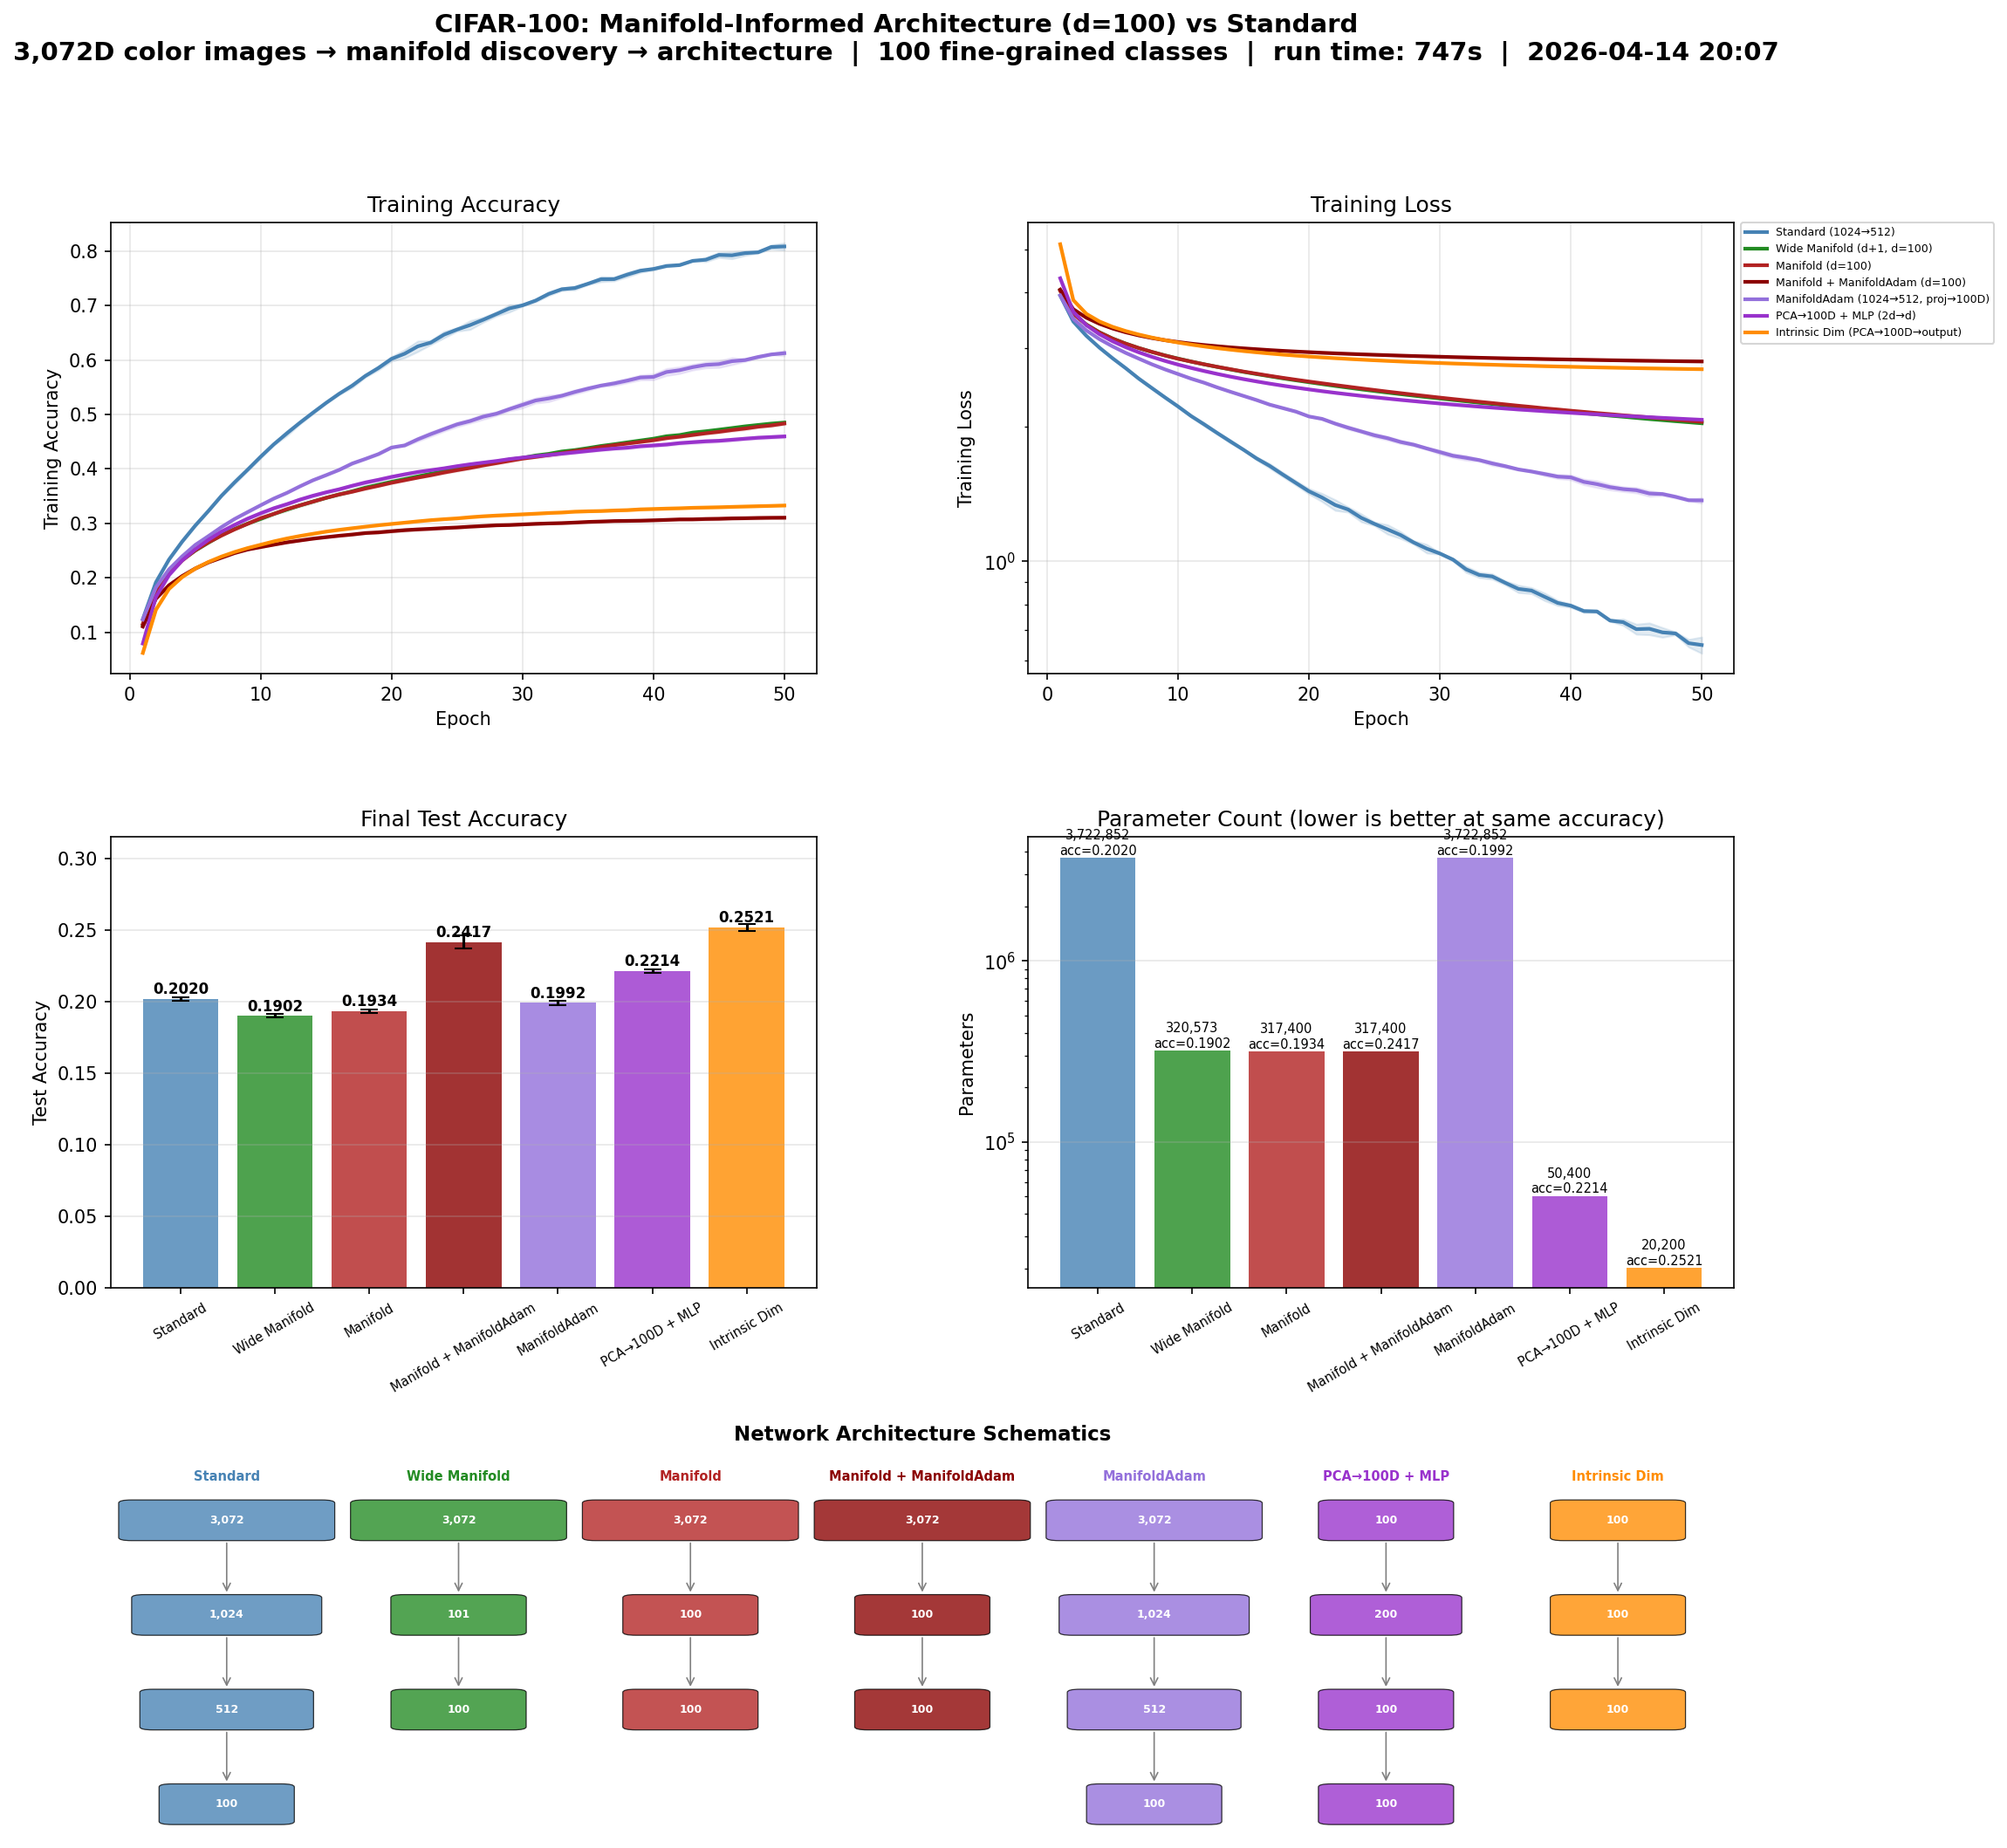
\includegraphics[width=\textwidth]{cifar100_architecture_results}
\caption{CIFAR100 manifold-informed vs.\ standard architecture comparison. $d = 19$, 100 epochs, 3 trials.}
\end{figure}

\section{Provenance}

\begin{tabular}{@{}ll@{}}
\toprule
\textbf{Item} & \textbf{Value} \\
\midrule
  Repository & \href{https://github.com/Flux-Frontiers/waverider}{Flux-Frontiers/waverider} \\
  Commit & \texttt{3c5d283} (--abbrev-re
3c5d28344fd5c5ace0b3399593d61b40363afcda) \\
  Commit date & 2026-08-04 03:22:44 +0000 \\
  Commit message & docs(readme): add holographic-rendering Breaking News section; audit fixes \\
  Python & 3.12.3 \\
  TensorFlow & 2.21.0 \\
  Device & CPU \\
  Host & vm \\
  OS & Linux-6.18.5-fc-v18-x86\_64-with-glibc2.39 \\
  Machine & Apple M5 Max MacBook Pro, 64 GB RAM, 2TB SSD \\
  Generated & 2026-08-04 03:29:45 \\
\bottomrule
\end{tabular}

\end{document}
